\documentclass[10pt,letterpaper]{article}
\usepackage[margin=0.75in]{geometry}
\usepackage{amsmath,graphicx,booktabs,float,caption}
\captionsetup{font=small,labelfont=bf}
\makeatletter\renewcommand\section{\@startsection{section}{1}{0pt}{-8pt}{3pt}{\normalfont\large\bfseries}}\makeatother
\setlength{\parskip}{3pt}
\title{\vspace{-1.2cm}Can your model A stop expanding and still fit? A bound-expansion fit}
\author{Addendum to the integrated model at $R=14.3$ Gpc}
\date{September 26, 2026}
\begin{document}
\maketitle\vspace{-0.9cm}

\section{Constraints}
We use the integrated fixed-profile model of the previous addendum, with its geometry, $e^{-r/L}$ profile, sine term and start at $0.01\,t_0$. The CoE mass and an optional uniform background of mass $M_b$ act on every particle through
\begin{equation}\label{eq:eom}
\ddot{\mathbf x}=-\frac{G\,[M(<r)+M_b(<r)]}{r^3}\,\mathbf x,\qquad M_b(<r)=M_b\,\min\!\left(1,\,r^3/D^3\right),
\end{equation}
and Earth's specific energy today uses the exact potential of both,
\begin{equation}\label{eq:E}
E=\tfrac12 v_E^2+\Phi(r_E),\qquad
\Phi(r)=-\frac{G M_{\rm tot}}{L}\left[\frac{f(u)}{u}+\frac{(1+u)e^{-u}}{2}\right]+\Phi_b(r),\qquad u=\frac rL,\quad M_{\rm tot}=\frac{M}{f(D/L)},
\end{equation}
with $f(u)=1-e^{-u}(1+u+u^2/2)$ and $\Phi_b=-GM_b(3D^2-r^2)/2D^3$ inside $D$, $-GM_b/r$ outside. A fit is accepted only if $E\le0$, so that Earth eventually turns around, and if every particle's radial velocity stays positive up to today. We quote the bound fraction as $(v_E/v_{\rm esc})^2=v_E^2/[-2\Phi(r_E)]$, which is at most 1 for a bound Earth. The turnaround time comes from continuing Earth's radial motion past today. The background is a uniform sphere of radius $D$ centred on the CoE and fixed in space. We did not let it expand with the flow, because comoving uniform matter in a flow with $H=1/t$ has a density parameter that grows as $t_0/t$ toward early times. At $\Omega_b=0.3$ that is 30 at the start, so everything recollapses long before today, which is the same ill-posedness that ruled out the comoving CoE profile. Truncating it at $D$ adds its mass to the mass inside $D$ and keeps its potential finite.

Migkas plot $A/A_{\rm all}$, the ratio to the all-sky mean. Your sheet instead divides by the unperturbed $kR$, which is harmless when gravity is weak but not when it is strong enough to bind. We therefore fit both forms,
\begin{equation}\label{eq:norm}
A_{\rm literal}(\theta)=\left[1-{\rm Amp}\sin(\theta+\varphi)\right]\frac{|\Delta\dot{\mathbf x}|}{kR},\qquad
A_{\rm sky}(\theta)=\left[1-{\rm Amp}\sin(\theta+\varphi)\right]\frac{|\Delta\dot{\mathbf x}|}{\langle|\Delta\dot{\mathbf x}|\rangle_{\rm sky}} .
\end{equation}
Only the combination $\mu=GMt_0^2/D^3$ enters the dynamics, so the age and the mass are degenerate. With $H_0=70$ km\,s$^{-1}$\,Mpc$^{-1}$ fixed as Earth's expansion rate today, each solution sets its own age and mass,
\begin{equation}\label{eq:age}
t_0=\frac{(Ht)_E}{H_0},\qquad (Ht)_E=\frac{v_E\,t_0}{r_E},\qquad M=\frac{\mu D^3}{G t_0^2},\qquad \frac{M}{M_{\rm crit}}=\frac{2\mu}{(Ht)_E^2}.
\end{equation}

\section{Results}
With your literal normalisation, no bound solution fits. Binding Earth requires deceleration of order the expansion itself, and that lowers every relative velocity together. The mean of your model A then drops well below the Migkas mean of 1, which ruins $R^2$ (dotted curve in Fig.~\ref{fig:r2}). The only way to be bound without that deceleration is to spread the mass far beyond $D$ ($L/D\approx2.5$), so that the potential is deep while the tidal pull on the shell is weak. That leaves almost no anisotropy, and $R^2$ falls to the level of the sine term alone (Table~\ref{tab:fit}). Adding the uniform background makes this worse.

Normalised to the sky mean, as Migkas's $A/A_{\rm all}$ is, the uniform part of the deceleration drops out. Bound solutions then fit as well as the unbound one, and slightly better (Table~\ref{tab:fit}). In fact the unconstrained sky-normalised optimum is already bound, so constraint (a) costs nothing. These solutions have about one critical mass inside $D$ with $L/D\approx0.52$--0.64 and $D/R\approx1.4$--1.6, and Earth turns around at 2.8--3.8 $t_0$. A background of $\Omega_b=0.3$ today takes over part of the binding, lowers the CoE mass to 0.63--0.83 critical, delays turnaround to 3.7--5.6 $t_0$ and costs less than 0.01 in $R^2$. Freeing $\Omega_b$ with $\ell_0$ also finds a branch with a large background and almost no CoE mass. Its anisotropy comes from the artificial edge of the background at $r=D$, so we do not regard it as physical.

The age is the tighter limit. Under attraction alone the expansion only slows, so $(Ht)_E<1$ always and $t_0<1/H_0=14.0$ Gyr. That also rules out any age of order $r/c=46.6$ Gyr without a repulsive term. The unrestricted bound optima have $(Ht)_E\approx0.79$--0.83, so they are 11.1--11.6 Gyr old and fall below the 12 Gyr oldest-star limit. They are flagged in Table~\ref{tab:fit}. Requiring an age of at least 12 Gyr as well, which means $(Ht)_E\ge0.859$, costs almost nothing. The fit moves to a lighter, more extended mass of about 0.66 critical ($L/D\approx0.44$) that is still bound, keeps $R^2=0.898$ with $\ell_0$, and turns around after about 8 ages, near 100 Gyr. With $\Omega_b\approx0.3$ the same holds at 0.44 critical, with turnaround after about 20 ages. Asking for 13 Gyr is too much: the best solution then sits exactly on the bound edge ($E=0$, turnaround only at infinity), and $R^2$ falls to 0.72. A bound universe with $H_0=70$ that fits the dipole can therefore just meet the oldest stars at 12 Gyr, but not 13 Gyr. This is the classic age problem of a decelerating universe.

\begin{table}[H]\centering\scriptsize\setlength{\tabcolsep}{2.6pt}
\caption{Constrained best fits, vs the Migkas points unless marked. All rows keep every particle moving outward today; ``bound'' adds $E\le0$ for Earth. $M/M_{\rm crit}$ and $\Omega_b$ are fractions of the critical mass inside $D$ at $H_0=70$ today. Age is $t_0$ from Eq.~(\ref{eq:age}), with a dagger for ages below 12 Gyr; the last block adds the age limit to the bound fit; turnaround is in units of that age. Rows with $(v/v_{\rm esc})^2=1$ sit on the bound edge and turn around only at infinity. The sky-normalised fits without the bound constraint are identical to the bound rows.}\label{tab:fit}
\begin{tabular}{lcccccccccccc}\toprule
Case & $D/R$ & $L/D$ & $M/M_{\rm crit}$ & $\Omega_b$ & $\ell_0$ [$^\circ$] & Amp & $\varphi$ & $R^2_{\rm Migkas}$ & $R^2_{A_F}$ & $(v/v_{\rm esc})^2$ & Age [Gyr] & Turnaround [$t_0$]\\\midrule
Literal, unbound allowed & 2.71 & 0.072 & 0.0248 & 0.00 & 0.0 & $-$0.052 & 0.51 & 0.755 & 0.829 & 34.5 & 13.7 & $\infty$\\
Literal, unbound allowed, $\ell_0$ & 2.90 & 0.070 & 0.0273 & 0.00 & 13.2 & $-$0.051 & 0.75 & 0.894 & 0.979 & 30.7 & 13.6 & $\infty$\\
\midrule
Literal, bound & 5.50 & 2.633 & 0.0367 & 0.00 & 0.0 & $-$0.052 & 0.57 & 0.277 & 0.307 & 1 & 13.9 & $\infty$\\
Literal, bound, $\ell_0$ & 5.45 & 2.428 & 0.0423 & 0.00 & 14.0 & $-$0.052 & 0.82 & 0.279 & 0.309 & 1 & 13.9 & $\infty$\\
Literal, bound, $\Omega_b=0.3$ & 1.05 & 3.000 & 0.0187 & 0.31 & 0.0 & $-$0.047 & 6.18 & $-$0.004 & $-$0.008 & 1 & 13.3 & $\infty$\\
\midrule
Sky-normalised, bound & 1.37 & 0.641 & 1.31 & 0.00 & 0.0 & $-$0.116 & 5.13 & 0.776 & 0.853 & 0.188 & 11.1$^\dagger$ & 2.80\\
Sky-normalised, bound, $\ell_0$ & 1.56 & 0.566 & 1.06 & 0.00 & 12.4 & $-$0.086 & 5.17 & 0.899 & 0.984 & 0.274 & 11.4$^\dagger$ & 3.39\\
Sky-normalised, bound, vs $A_F$ & 1.36 & 0.570 & 1.12 & 0.00 & 0.0 & $-$0.116 & 5.13 & 0.776 & 0.853 & 0.255 & 11.3$^\dagger$ & 3.23\\
Sky-normalised, bound, vs $A_F$, $\ell_0$ & 1.52 & 0.524 & 0.963 & 0.00 & 12.3 & $-$0.088 & 5.16 & 0.899 & 0.985 & 0.331 & 11.5$^\dagger$ & 3.83\\
\midrule
$\Omega_b=0.3$, bound & 1.34 & 0.490 & 0.832 & 0.30 & 0.0 & $-$0.120 & 5.12 & 0.772 & 0.852 & 0.348 & 11.4$^\dagger$ & 3.70\\
$\Omega_b=0.3$, bound, $\ell_0$ & 1.50 & 0.442 & 0.701 & 0.30 & 12.6 & $-$0.091 & 5.14 & 0.895 & 0.983 & 0.444 & 11.5$^\dagger$ & 4.63\\
$\Omega_b=0.3$, bound, vs $A_F$ & 1.33 & 0.435 & 0.709 & 0.30 & 0.0 & $-$0.119 & 5.12 & 0.771 & 0.852 & 0.443 & 11.5$^\dagger$ & 4.60\\
$\Omega_b=0.3$, bound, vs $A_F$, $\ell_0$ & 1.48 & 0.408 & 0.631 & 0.30 & 12.3 & $-$0.092 & 5.14 & 0.895 & 0.983 & 0.516 & 11.6$^\dagger$ & 5.60\\
\midrule
$\Omega_b$ free, bound, $\ell_0$ (edge branch) & 2.19 & 0.068 & 0.00277 & 5.31 & 192.1 & $-$0.150 & 4.46 & 0.903 & 0.971 & 0.113 & 8.7$^\dagger$ & 1.54\\
\midrule
Age $\ge12$ Gyr & 1.45 & 0.436 & 0.664 & 0.00 & 0.0 & $-$0.090 & 5.26 & 0.773 & 0.850 & 0.604 & 12.0 & 8.32\\
Age $\ge12$ Gyr, $\ell_0$ & 1.66 & 0.436 & 0.664 & 0.00 & 12.5 & $-$0.067 & 5.31 & 0.898 & 0.983 & 0.604 & 12.0 & 8.33\\
Age $\ge12$ Gyr, vs $A_F$, $\ell_0$ & 1.59 & 0.421 & 0.652 & 0.00 & 12.4 & $-$0.072 & 5.27 & 0.898 & 0.984 & 0.634 & 12.0 & 9.30\\
$\Omega_b\approx0.3$, age $\ge12$ Gyr & 1.42 & 0.351 & 0.444 & 0.28 & 0.0 & $-$0.094 & 5.24 & 0.768 & 0.849 & 0.781 & 12.0 & 18.55\\
$\Omega_b\approx0.3$, age $\ge12$ Gyr, $\ell_0$ & 1.60 & 0.346 & 0.44 & 0.28 & 12.7 & $-$0.071 & 5.27 & 0.894 & 0.982 & 0.792 & 12.0 & 20.12\\
$\Omega_b\approx0.3$, age $\ge12$ Gyr, vs $A_F$, $\ell_0$ & 1.54 & 0.333 & 0.43 & 0.28 & 12.4 & $-$0.076 & 5.24 & 0.893 & 0.982 & 0.82 & 12.0 & 24.85\\
Age $\ge13$ Gyr, $\ell_0$ & 4.03 & 0.584 & 0.332 & 0.00 & 14.4 & $-$0.042 & 0.56 & 0.719 & 0.789 & 1 & 13.0 & $\infty$\\

\bottomrule\end{tabular}\end{table}

\begin{figure}[H]\centering
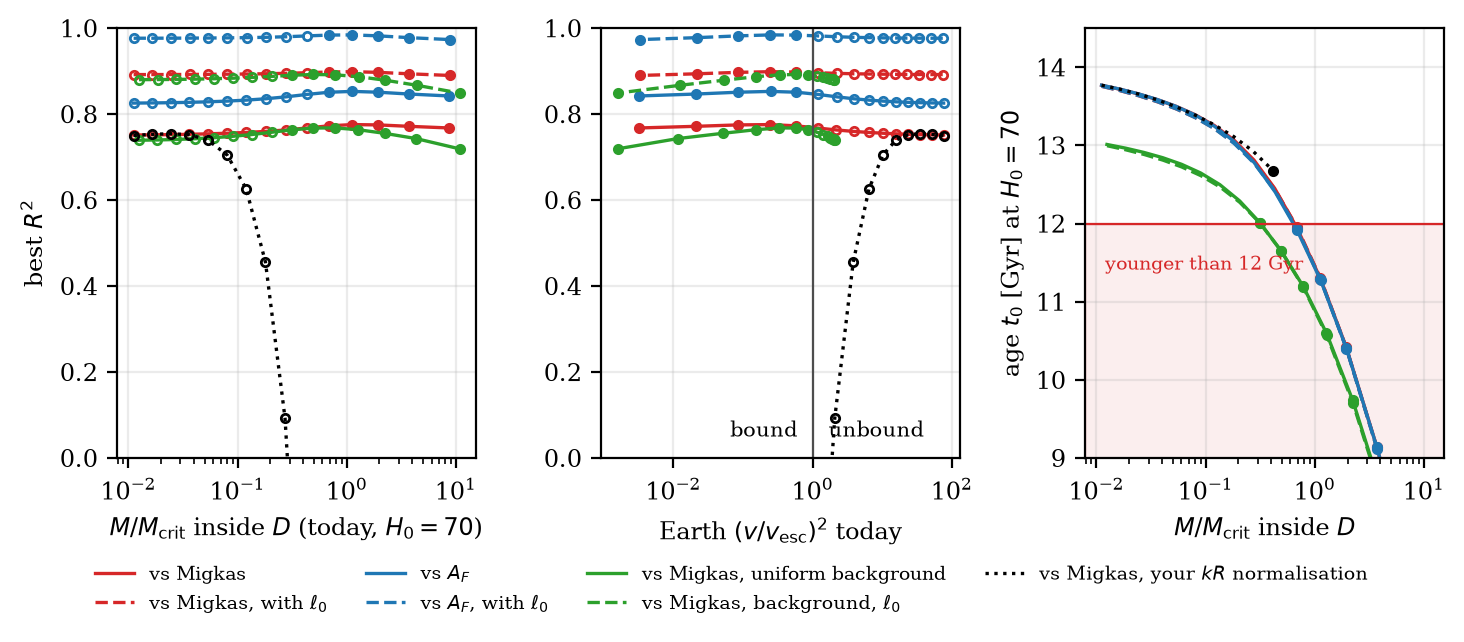
\includegraphics[width=0.92\textwidth]{bound_fit_R2.png}
\caption{Best $R^2$ with $D/R$, $L/D$, Amp and $\varphi$ (and $\ell_0$ where marked) re-fitted at each CoE mass, sky-normalised except the dotted curve. Filled points have a bound Earth. The green curves add a uniform background of 0.3 critical at the unperturbed rate, which is about 0.45 at today's rate. The right panel gives the age at $H_0=70$; the shaded band is younger than the oldest stars. Curves end where particles turn around before today.}\label{fig:r2}
\end{figure}
\end{document}
